\chapter{Harvesting The Fruits of Uncertainty}
\label{chapter_3lab}

The first study of a pineapple leaf valorisation process published in Costa Rica is a dissertation by \cite{quesada2003utilizacion}, who analyses the use of PAL as a polyester resin reinforcement. Since then, numerous studies in the natural and social sciences related to PAL valorisation processes have been published in Costa Rica and elsewhere. Yet, after two decades of the creative dissertation's publication, the valorisation of PAL has not taken off in Costa Rica. 

This chapter is devoted to explaining the complexity of the system in which the valorisation of PAL in Costa Rica occurs. To advance in the implementation of valorisation, we first need to understand why valorisation has not taken place and what are the barriers preventing it. Only then we can theorise what can be done to bring down those barriers and which stakeholders can lead the way in the circular economy.

\section{Theories on Circular (Bio)Economy}
\label{theoryframe}

 Due to the novelty of PAL valorisation and the complexity of the system in which it takes place, it is appropriate to define the concepts and discuss the theories that relate to the subject under study. There are several interlinked concepts we find relevant to discuss: the circular economy, the bioeconomy, the intersection of the last two, and the circular economy in the agricultural sector. Additionally, we discuss theories that serve to delineate the scope of our study.  Drawing from \cite{gottinger2020studying}, we describe how the Technological Innovation Systems (TIS) and similar frameworks can be used to identify the factors influencing transitions to a circular (bio)economy. The analytical framework designed by \cite{blomsma2022making} based on action recipes helps us to understand how circular-oriented innovation (COI) processes unfold.

\paragraph{Circular Bio(Economy)} \mbox{}\\
 The definition of circular economy varies in the literature and \cite{kalmykova2018circular} present the commonalities found among them. The first commonality is the maximisation of the value of the resources in use, also called stock optimisation. Eco-efficiency is also commonly mentioned when defining CE, sometimes as a consequence of it, other times as a purpose, and in some cases as a synonym. Yet, the authors remind us that eco-efficiency can also be achieved in a linear economy and that CE should rather aim to be eco-effective. The latter focuses not only on minimising the cradle-to-grave flow of materials but also on generating cyclical, cradle-to-cradle processes. Another concept often mentioned is waste prevention, which is frequently presented as the main purpose of CE. Finally, the four Rs (Reduce, Reuse, Recycle and Recover), the mechanism for achieving CE, is another shared feature among the CE definitions. 

There are also differences between the definitions that relate to the tightness of the loop within a value chain, that is, how closely the phases should be, and to the scope, which refers to the included resources: all physical resources or only certain sectors, products, materials, and substances. Because of these differences and because the shared features are not present in all definitions, \citeauthor{kalmykova2018circular} conclude that there is no established common ground for the variety of existing CE conceptualisations. Essentially, CE is a combination of several sustainability concepts and draws on other sustainability fields to construct its strategies. 

The concept of bioeconomy is commonly used alongside that of the circular economy. Their relationship and their differences as noted by \cite{carus2018circular} serve useful in our framework. Bioecomy involves the production of renewable biological resources and their conversion into value-added products, such as food, feed, biobased products, and bioenergy. The objectives of the bioeconomy are the introduction of healthy, safe and nutritious food and animal feed; the provision of bioenergy and biofuels to replace fossil energy; the development of new, more efficient, and sustainable agricultural and marine practices, the mitigation of climate change through the substitution of petrochemicals by materials with lower GHG emissions, and fossil fuels by biofuels; and the emergence of new business opportunities, investment and employment to rural, coastal and marine areas, fostering regional development and supporting small and medium enterprises.

Both the bioeconomy and the circular economy aim to avoid the use of additional fossil fuels and to a more resource-efficient system. As \cite{carus2018circular} clarify, the circular economy and the bioeconomy are two different yet complementary approaches to promoting sustainability. The circular economy focuses on improving resource efficiency and reducing the use of fossil fuels by incorporating recycled materials into processes. Bioeconomy aims to replace fossil fuels with biomass derived from agriculture, forestry, and marine environments. The intersection between the two concepts, the circular bioeconomy, can be interpreted in many ways. \cite{tan2021circular} mention that the relationship between CE and bioeconomy is complex and explain that the circular bioeconomy is more than the intersection of both concepts, their combination results in a more sustainable framework. Perhaps more useful is to look at their limitations to understand their differences. CE focuses on economic and environmental benefits while ignoring the social dimension. Moreover, efficiency gains can be confronted with rebound effects in the form of increased production and consumption. As for the bioeconomy, this cannot bring the perceived environmental benefits only by substituting fossil-based resources with bio-based ones.

It is important to note that both the CE and the bioeconomy are focused on resources, i.e., they deal with the cycle of materials, but they ignore the relationship between this cycle and broader ecological processes and ecosystem services such as water, nutrient cycles, quality of the energy source, and protection of biodiversity and ecosystems. In this sense, we find relevant the study by \cite{velasco2021circular} on CE in the agricultural sector. As the authors define it, apart from the components of the CE defined above, the CE in agriculture should also guarantee the regeneration of biodiversity in agroecosystems and the surrounding ecosystems. Additionally, they identify the main differentiating characteristics that must be considered in a CE framework for the agricultural sector. These are the perishable nature of products, the close link with natural ecosystems, and the strong seasonality of production. 


\paragraph{Transition towards a Circular Bioeconomy} \mbox{}\\
In their literature review, \cite{gottinger2020studying} provide an analysis of the different theoretical frameworks used to study the transition towards circular bioeconomy (CB). They conclude that the Technological Innovation Systems (TIS) framework has empirically served as most useful to identify influential factors to transition. \cite{markard2008technological} define TIS as \textit{a set of networks of actors and institutions that jointly interact in a specific technological field and contribute to the generation, diffusion and utilisation of variants of a new technology and/or a new product}. Actors can be individuals, companies, or governmental and non-governmental organisations. Institutions are the regulations and norms that influence the actions, decisions, and processes of actors. The networks can be learning networks that create knowledge bridges, or they can be policy networks linking actors with the same beliefs and agenda. In TIS, barriers are called blocking mechanisms, which hinder technology diffusion and industry development. The concept of system weaknesses is also commonly used in the framework and is usually the focus of the analysis when considering policy interventions \citep{giurca2017forest}.

Most studies assessing the CB transition analyse the strengths and weaknesses of innovation systems, the impact of certain events on the transition, and the facilitators of the transition. Less often, studies analyse the stakeholders, their roles and expectation towards the transition, and the interaction among them. A group of studies also focus on the changes that occur within existing sectors and their role in the transition. Finally, policies and their effects were studied in specific countries or by comparing policies cross-nationally.

\citeauthor{gottinger2020studying} identify six categories commonly found in the literature of barriers to transition toward CB.  
First, \textit{Policy and Regulation} is related to barriers associated with existing or missing policies and regulation implementation problems.
The category of \textit{Technology and Materials} encompasses the technical challenges associated with the application of technology and the creation of products, as well as the availability of input materials and physical infrastructure. 
\textit{Market and Investment} conditions refer to obstacles related to market demand and creation and the mobilisation and availability of financial resources. \textit{Social Acceptance} includes barriers associated with public awareness, interest and participation, as well as opposition from the public. \textit{Knowledge and Networks} encompass barriers linked to generating and applying knowledge, as well as the existence and development of efficient networks. Finally, \textit{Sectoral Routines and Structures} contains barriers associated with willingness and restrictiveness to change, such as risk-averse attitudes. From the analysed frameworks, TIS discovers a more extensive range of subcategories.

\paragraph{Circular-Oriented Innovation (COI)} \mbox{}\\
A big challenge in achieving a circular bioeconomy is to find ways to maximise the use of resources and, at the same time, convert them into value-added products. Thus, innovation plays a crucial role in driving the transition to a circular economy, as it enables the development of new, more sustainable, eco-efficient, and hopefully eco-effective, business models and processes. In this sense, \cite{blomsma2022making} explain how the processes of circular-oriented innovation (COI) occur. They draw from different organisation science frameworks to examine what strategies COI practitioners find relevant and how they employ CE action recipes, i.e., relationships between concepts and actions that help to clarify how ambiguity is addressed to enable action. They structure their framework by asking the following questions: 1) What is the motivation to engage in COI? (Which residues are present and where are they?), 2) How are circular strategies visualised to address the perceived issues? (Which circular strategies are applied and where?), 3) Who should act to implement them? (Which actors?).

Surprising or not, \citeauthor{blomsma2022making} find that the motivation to engage in COI consists of a complex mix of factors. CE solutions aim to address multiple problems, often in the form of structural wastes where there is lack of closing loops and preventative strategies. Additionally, CE practitioners identify benefits, such as larger profit margins or uncoupling from raw materials that will be scarce in the future. Answering the second question, they mention that circular strategies require linking knowledge and stakeholders in a manner not previously employed in the linear economy. Because circular strategies in complex real-life cases are not usually employed individually and instead interact with each other, an understanding of these synergies is required. This relates to the fact that CE is an umbrella term that, as mentioned before and explained by \cite{kalmykova2018circular}, draws from different sustainability strategies. Finally, the answer to which action is needed to implement CE solutions is focused on value network dependencies. The difficulties that COI practitioners face as CE strategies progress are related to the dependence on other actors within the system. Additionally, \cite{blomsma2022making} remark on the importance of deciding when stakeholders should be involved in innovation processes. Early engagements can hinder certain CE solutions, and sometimes it is best to wait until a solution is better developed to seek collaborations. Finally, by identifying the CE action recipes, some of the barriers initially defined as important by practitioners can be discarded later in favour of fewer but more central barriers. By focusing on a subset of barriers, innovators can take action more easily, which also allows them to take further steps more easily in the future. Nevertheless, this idea raises the question of when a circular solution can be considered to be sufficiently developed. In this sense, the authors recommend taking a sufficiently long time horizon to understand circular phenomena in business. 

As mentioned above, value network dependencies play a relevant role in COI implementation. Therefore, we find it useful to look into how collaboration takes place in COI more deeply. \cite{brown2019companies} provide an insight into the motives, barriers and drivers that stimulate or hamper collaborative innovation within the context of CE. They divide the identified motives into intrinsic (realised for their own sake), and extrinsic (realised for external recognition). Both can originate from the personal and organisational levels. For example, responsibility for sustainability can have intrinsic and extrinsic motives, and such motives trigger collaboration with other actors if both parties feel alignment between their motivations. Moreover, the recognition of interdependence also stimulates collaboration. The complexity of CE strategies and the dispersion of knowledge among stakeholders drives this interdependence. 

Another motive driving collaboration is the necessity to find suitable experimental arrangements. These arrangements break down complex systems into manageable projects. Then, experimentation helps in creating knowledge, and in engaging stakeholders to develop evidence that helps overcome barriers to adopting CE strategies. Testing at scale is important to identify unintended or unexpected impacts in the system, and collaboration is necessary to share the potential risks and costs. The last motive that stimulates collaboration identified by \citeauthor{brown2019companies} is the need to implement the business model. This motive is not as developed because technical innovation is usually more advanced than market/business model innovation. Collaboration is needed to develop all the operations required for CE strategies, but there is less collaboration in this area due to competition. In this sense, a clear barrier to collaboration in the context of COI is the contradiction of companies wanting to share but also protect knowledge. Moreover, sharing economic rewards becomes more difficult as companies prioritise individual returns over the shared benefits drawn from the project. This creates a cultural barrier that can hinder the progress of collaborative innovation efforts beyond the experimental phase. 

If the culture in the organisations involved in COI is not aligned, the shared CE objectives will not develop. The challenge is to increase internal motivation and change culture before even achieving evidence of CE. As concluded by the \citeauthor{brown2019companies}, COI is confronted with the challenge of transitioning from exploring new market opportunities and closed-loop experiments to initiating societal transformations through larger-scale collaborations. This necessitates overcoming barriers related to organisational mindsets and collaborative knowledge sharing. The latter requirement is a shared concept among CE frameworks. For example, \cite{antikainen2016framework} highlight the importance of the interaction between stakeholders when building CE business models. Their study corroborates the idea that CE business models are not isolated but rather integrated into a system of business models that together close a material loop. COI, in this sense, requires the collaboration and communication of many parties.

Inventions do not necessarily bring innovation. When we analyse the valorisation of PAL, we can think of it merely as the invention of a new product and the recycling of agricultural residues, or we can see it as part of an innovation process driven by many stakeholders for a sufficiently long period to transition to a more circular economy. Whether PAL valorisation remains an invention or progresses to become an innovation depends on the capacity of the industry and stakeholders to overcome the barriers preventing its implementation and to exploit its linkages to the circular bioeconomy revolution.

\begin{comment}
....................

Technology acceptance model: This theory can be used to understand the factors that influence the adoption and usage of new technology. In the context of transitioning to circular management of pineapple stubble, the technology acceptance model can be used to identify the technological and cultural barriers that prevent stakeholders from adopting and utilising circular practices.

Resource dependence theory: This theory can be used to explain how organisations are dependent on their environment for resources and how they manage their dependencies. In the context of pineapple stubble, resource dependence theory can be used to understand the interdependencies of actors in the industry and how they may affect the adoption of circular practices.

Institutional theory: This theory can be used to explain how institutional norms and values shape the behaviour of actors in an industry. In the case of pineapple stubble, institutional theory can be used to understand how cultural beliefs and practices, as well as regulatory frameworks, may inhibit the adoption of circular practices.

Socio-technical systems theory: This theory can be used to understand the interactions between social and technical components of a system and how they influence each other. In the context of pineapple stubble, socio-technical systems theory can be used to understand how social, cultural, and technical factors interact to prevent the adoption of circular practices.

Prospect theory: This theory explains how people make decisions under risk and uncertainty. In the context of pineapple stubble, prospect theory can be used to understand how risk-taking aversion among companies may inhibit the adoption of circular management practices.

Real options theory: This theory can be used to understand how firms make investment decisions under uncertainty. In the context of pineapple stubble, real options theory can be used to understand how companies may perceive the uncertainty of the benefits of adopting circular management practices as a barrier to their adoption.

Innovation adoption model: This theory can be used to understand the factors that influence the adoption of innovations by organisations. In the context of pineapple stubble, the innovation adoption model can be used to identify the factors that influence the adoption of circular management practices, including the perceived risks and uncertainties associated with the transition.

\end{comment}

\section{Methodology}

\subsection{Fuzzy Cognitive Maps for Knowledge Elicitation and Analysis}

A lot of knowledge is created in the process of innovation. Many times, this knowledge can be dispersed, or fuzzy. The fuzzier the knowledge representation, the easier the knowledge acquisition, but also the harder the knowledge processing. In such cases, Fuzzy Cognitive Mapping (FCM) serves as a great tool for eliciting this fuzzy knowledge because it allows fuzzy degrees of causality between causal concepts \citep{kosko1986fuzzy}. 

FCM is a technique that builds quasi-quantitative models from the knowledge of interconnected variables in a system. It was first introduced by \cite{kosko1986fuzzy}, who presented FCM as a tool to model complex systems and decision-making. Fuzzy Cognitive Maps are composed of a set of nodes that represent the variables or concepts of the system and a set of links between them that represent the relationships between the variables. Each link is associated with a weight that represents the strength of the relationship between the variables. These weights can be positive or negative and, thus, variables can ``decrease'' or ``increase''. A simple example of an FCM with three concepts and four connections is presented in \cref{example_fcm}. The connections between the variables in the system represent causal influence. Exploring how these causal influences propagate through the system when it is subject to change or intervention is the main objective of FCM \citep{barbrook2022systems}.

\begin{figure}[H]
\caption{Example of a Fuzzy Cognitive Map}  
\label{example_fcm}
\centering
\includesvg[inkscapelatex=false,width=8cm]{fig/fuzzyExample.svg}
\end{figure}

There are two main approaches to using FCM. The ``causal" approach implies that the strength of links between concepts represents how certain the experts are that a factor causes, or suppresses, another. The ``dynamical" approach models the propagation of effects of one concept on another, resulting in a representation of the relative magnitude of changes in concept values. This approach allows us to understand which concepts are the most important or the most influenced in a system. In our study, we use the dynamical approach because it reflects a widespread usage of FCM in a participatory manner and allows for a better interpretation of cognitive maps.

The FCM modelling technique allows for more nuanced modelling of relationships that better reflect the uncertainty and ambiguity that are often present in real-world systems. As \cite{ozesmi2004ecological} explain, FCM can involve local people who typically possess a comprehensive understanding of the ecosystem and whose participation and input can be crucial for informed decision-making and for gaining acceptance from the public for the proposed solutions. Furthermore, ``wicked" environmental problems that involve many stakeholders and which have no easy solutions can benefit from a model that brings together the knowledge of different experts from different disciplines and compares their perceptions. In this way, FCM can help to understand the advantages and disadvantages of possible decisions. Finally, it is important to highlight the benefits of the interaction between the researcher and the stakeholders throughout the analysis. As a participatory approach, FCM allows for recursive feedback, which helps to model an accurate representation of reality. Moreover, this approach provides the stakeholders with the opportunity to reflect on the problem at hand; the process of building a Fuzzy Cognitive Map is as important as its results. 

The use of FCM in the field of environmental studies is extensive, covering climate change \citep{kontogianni2012you, singh2014livelihood, reckien2014weather}, deforestation \citep{kok2009potential}, fire ecology \citep{devisscher2016anticipating, eriksson2022using}, pollution \citep{anezakis2016fuzzy, salberg2022assessing, ozesmi2003participatory}, renewable energy \citep{jetter2011building, alipour2019characteristics, kyriakarakos2014fuzzy}, urban ecology \citep{assunccao2020rethinking, olazabal2016use}, water use \citep{giordano2005fuzzy, kafetzis2010using}, and waste management \citep{falcone2020use, morone2021using, kokkinos2018fuzzy, konti2018exploring}. 

There are many ways of developing and applying Fuzzy Cognitive Maps, but the structure is regularly the same. We find that the six steps proposed by \cite{edwards2021building} and illustrated in \cref{stepsFCM} are suitable for our case. The authors implement an episodic and asynchronous method with the participation of stakeholders on two occasions. The process starts by determining the scope and objective of the study, which results in the design of an interview outline. The second step is the selection of stakeholders. Then, stakeholders are consulted to generate knowledge by means of in-depth individual interviews. The fourth step consists of the qualitative aggregation of concepts, in which the interviews' output is analysed and harmonised. In the fifth step, stakeholders participate for the second time to weigh the connections identified in the previous step, resulting in individual fuzzy cognitive maps. The last step involves combining the responses to generate the aggregated FCM and further analyse it. In the following sections, the implantation of these steps for our case is explained in detail.

\begin{table}[H]
\centering
\resizebox{\textwidth}{!}{
\begin{threeparttable}
\caption{Fuzzy Cognitive Map Building Steps and Products}
\label{stepsFCM}
\begin{tabular}{lll} \hline \hline 
       & Process                           & Product                                            \\ \cline{2-3} 
Step 1 & Definition of objective and scope & Interview Questions                                \\
Step 2 & Stakeholder selection             & List of Participating Stakeholders                 \\
Step 3 & Knowledge generation              & Original concepts and connections                  \\
Step 4 & Qualitative aggregation           & Generalised labels for concepts, added connections \\
Step 5 & Weighting connections             & Individual FCMs                \\
Step 6 & Quantitative aggregation          & Aggregated FCM   \\ \hline   \hline     
\end{tabular}

\begin{tablenotes}
      \small \item Adapted from \cite{edwards2021building}
\end{tablenotes}
\end{threeparttable}%
}
\end{table}


\subsection{Definition of objective and scope}

We begin by defining the objective and scope of the FCM study which, as explained by \cite{edwards2021building}, guide both stakeholder identification and the questions posed to elicit knowledge about the system. In this chapter, we try to achieve the first objective defined in the Introduction: to understand why the valorisation of PAL has not taken off in Costa Rica. Thus, the scope, which refers to the study area we try to describe, is at the national level. The main question is \textit{What are the barriers preventing the valorisation of PAL in Costa Rica?} Thus, PAL valorisation is the first and central concept of the FCM. Finally, we define the interview questions to be asked to the stakeholders in the third step. It was decided to formulate open-ended questions to allow the interviewees to elaborate on their answers; this is often the domain of qualitative research \citep{barbrook2022systems}. The interview template is shown in \cref{interviewOutline}.
  
\subsection{Stakeholder selection}

When implementing FCM, it is important to represent all the people who impact or are affected by the system under study. A good way to determine whether the population to be represented has been sampled sufficiently is to check the number of new concepts added by each new participant. \cite{ozesmi2004ecological} examined accumulation curves of the total number of variables versus the number of interviews, as well as the number of new variables added per interview, using Monte Carlo techniques. Their results, depicted in \cref{accumFCM}, show that as the number of interviews increases, the number of new variables decreases and that the total number of variables increases at a decreasing rate. This behaviour is normal if we consider that most stakeholders in the system share the same vocabulary about the subject of enquiry. A similar result can be found in \cite{morone2021using}, whose research demonstrates how the generation of new variables decreases rapidly. However, \cite{ozesmi2004ecological} note that we can expect one or two new variables to be mentioned for each new interview. 

\begin{figure}[ht]
\caption{Accumulation curves of concepts versus interviews} \label{accumFCM}
\begin{subfigure}[b]{0.45\textwidth}
  \centering
  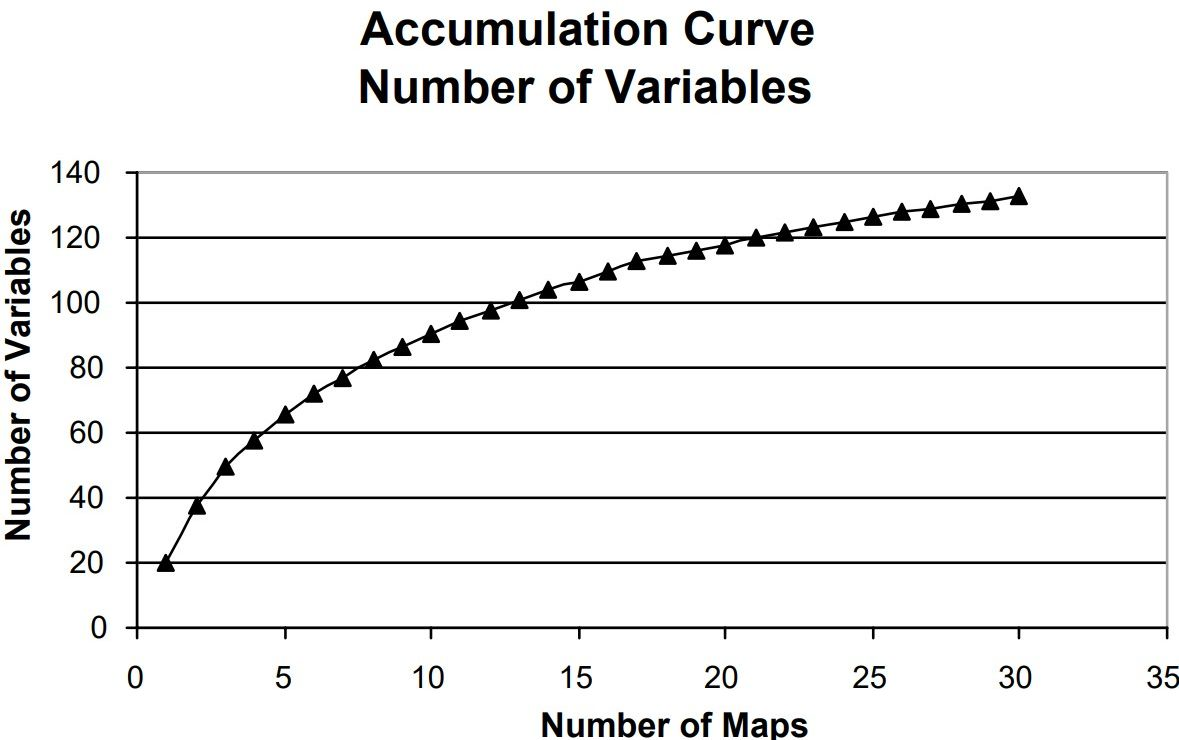
\includegraphics[width=\textwidth]{fig/numVars.jpg}
\caption{Number of variables vs. number of maps} 
  \label{accumFCM:sub1}
\end{subfigure}%
  \hfill
\begin{subfigure}[b]{0.45\textwidth}
  \centering
  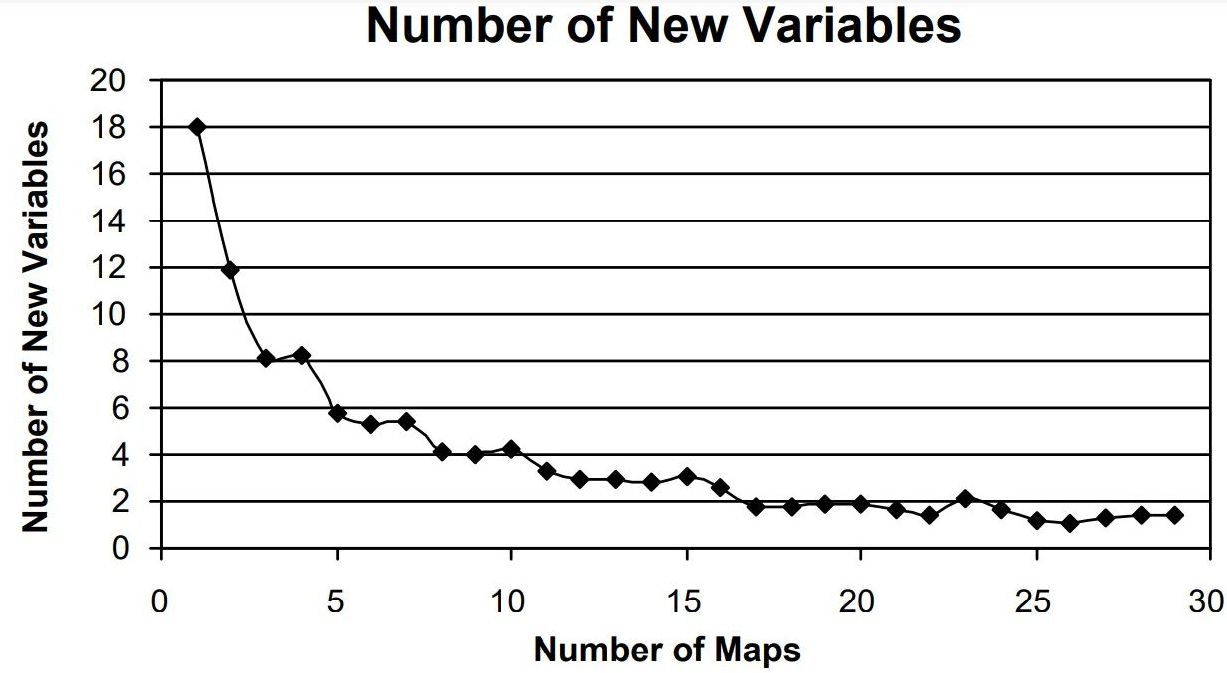
\includegraphics[width=\textwidth]{fig/newVars.jpg}
\caption{Number of new variables added per map}    
  \label{accumFCM:sub2}
\end{subfigure}
%\captionsetup{justification   = raggedright, singlelinecheck = false}
\caption*{\textit{Source:} \cite{ozesmi2004ecological}}
\end{figure}

It is useful to think of categories when selecting stakeholders in the system, and then identify individuals who fit the categories. As such, in our case study, we defined three broad categories: research, government, and industry. Once contact was made with an individual within each category, more participants were identified by snowballing. 

\subsection{Knowledge generation}

\cite{edwards2021building} highlight how important it is that the researcher designs and executes stakeholder engagement during their participation in the knowledge elicitation process so that their perspective is represented in the final product of the FCM. At this stage, the researcher decides the balance of coproduction, i.e., how much stakeholder input and researcher input are used in the process. Semi-structured in-person interviews were held separately with each identified stakeholder. It is important to have a structured interview process that allows for the collection of detailed information, while also giving the interviewee the freedom to share the information they deem most important. In the interviews, the stakeholders were first introduced to the objective and scope of the study. Then, the predefined questions were asked and, depending on the interviewees' responses, additional questions were posed to clarify or augment the information provided. No concepts were provided to stakeholders, but it was ensured that the focus was kept on the valorisation of PAL. The interview sessions lasted between 40 and 120 minutes, were conducted between August and November 2022, and were recorded when the respondents gave their consent. 

\subsection{Qualitative aggregation}

The recording of the interviews was transcribed using Whisper, a general-purpose speech recognition model. The script used for the transcription can be found in the Supplementary Material. The transcription of the interviews along with the notes taken by the researcher was used to create a list of concepts mentioned by the participants. In cases in which the interviewees defined the same concept using different vocabulary, the definitions were grouped into one concept. As concepts were identified, connections were established as well. 

In \cref{process_fcm} we demonstrate how the following statement made by one of the stakeholders was converted into four concepts and three connections: ``[W]hat we are looking for with the recovery of stubble is ... converting something that today is waste into a value-added product. [A]n economic benefit, but also a social and environmental benefit. For example, if we avoid the fly problem, we already have an important environmental benefit." This is a straightforward example, as it includes the central subject of study, the valorisation of PAL, and its main consequences. 

In the figure, it can be observed how vocabulary harmonisation and concept grouping take place. In the first step, identified concepts and connections between them are extracted from the interviewee's statement. Then, the concepts \textit{Recovery of stubble} and \textit{Value-added products} are grouped into \textit{PAL valorisation}. \textit{Economic benefit} is translated into \textit{Increase profitability of the pineapple producers} because producers are assumed to be the ones that valorise PAL in most cases and because economic benefits is a broad concept that has a different definition for different stakeholders. For the second round of stakeholders' participation, it is important to use clear concepts that convey a similar definition to everyone. For this harmonisation process, analysis of commonly used terms used in the literature is also useful. The same explanation is valid for the translation of \textit{Environmental benefits} into \textit{Increase Community’s Health/Wellbeing}. 

In the third step, it can be observed how the concepts take their final shape. The impact previously denoted in words, increase and reduce, are now connections, represented by positive and negative signs. It is worth noting how this affects the relation between concepts: in step two, the community's health/well-being is enhanced because the stable fly is avoided as PAL valorisation takes place. In the FCM, this is represented by two negative effects, one from the valorisation of PAL to the propagation of the stable fly, and another from the latter to the community’s health/wellbeing. In this way, the effect of PAL valorisation on the community’s health/wellbeing is transmitted through a negative effect to and from the (presence of) stable fly. This simple example also shows how important it is to use concepts that behave like variables, i.e., that can be thought to increase or decrease. 

The concepts and connections shown in \cref{process_fcm} are only part of the FCM built for our case, and the displayed concepts can affect or be affected by many other concepts. The aggregation and harmonisation process exemplified here needs to be repeated by revisiting statements and checking the logic and internal consistency within the concepts and connections. As more statements from different stakeholders are analysed, concepts are renamed, and connections are added or deleted. Finally, we find a map that represents how stakeholders perceive the system dynamics and that can be understood with ease. 

\begin{figure}[H]
\caption[Example of interview statement processing]{Example statement processing to build FCM concepts and connections}
\label{process_fcm}
\centering
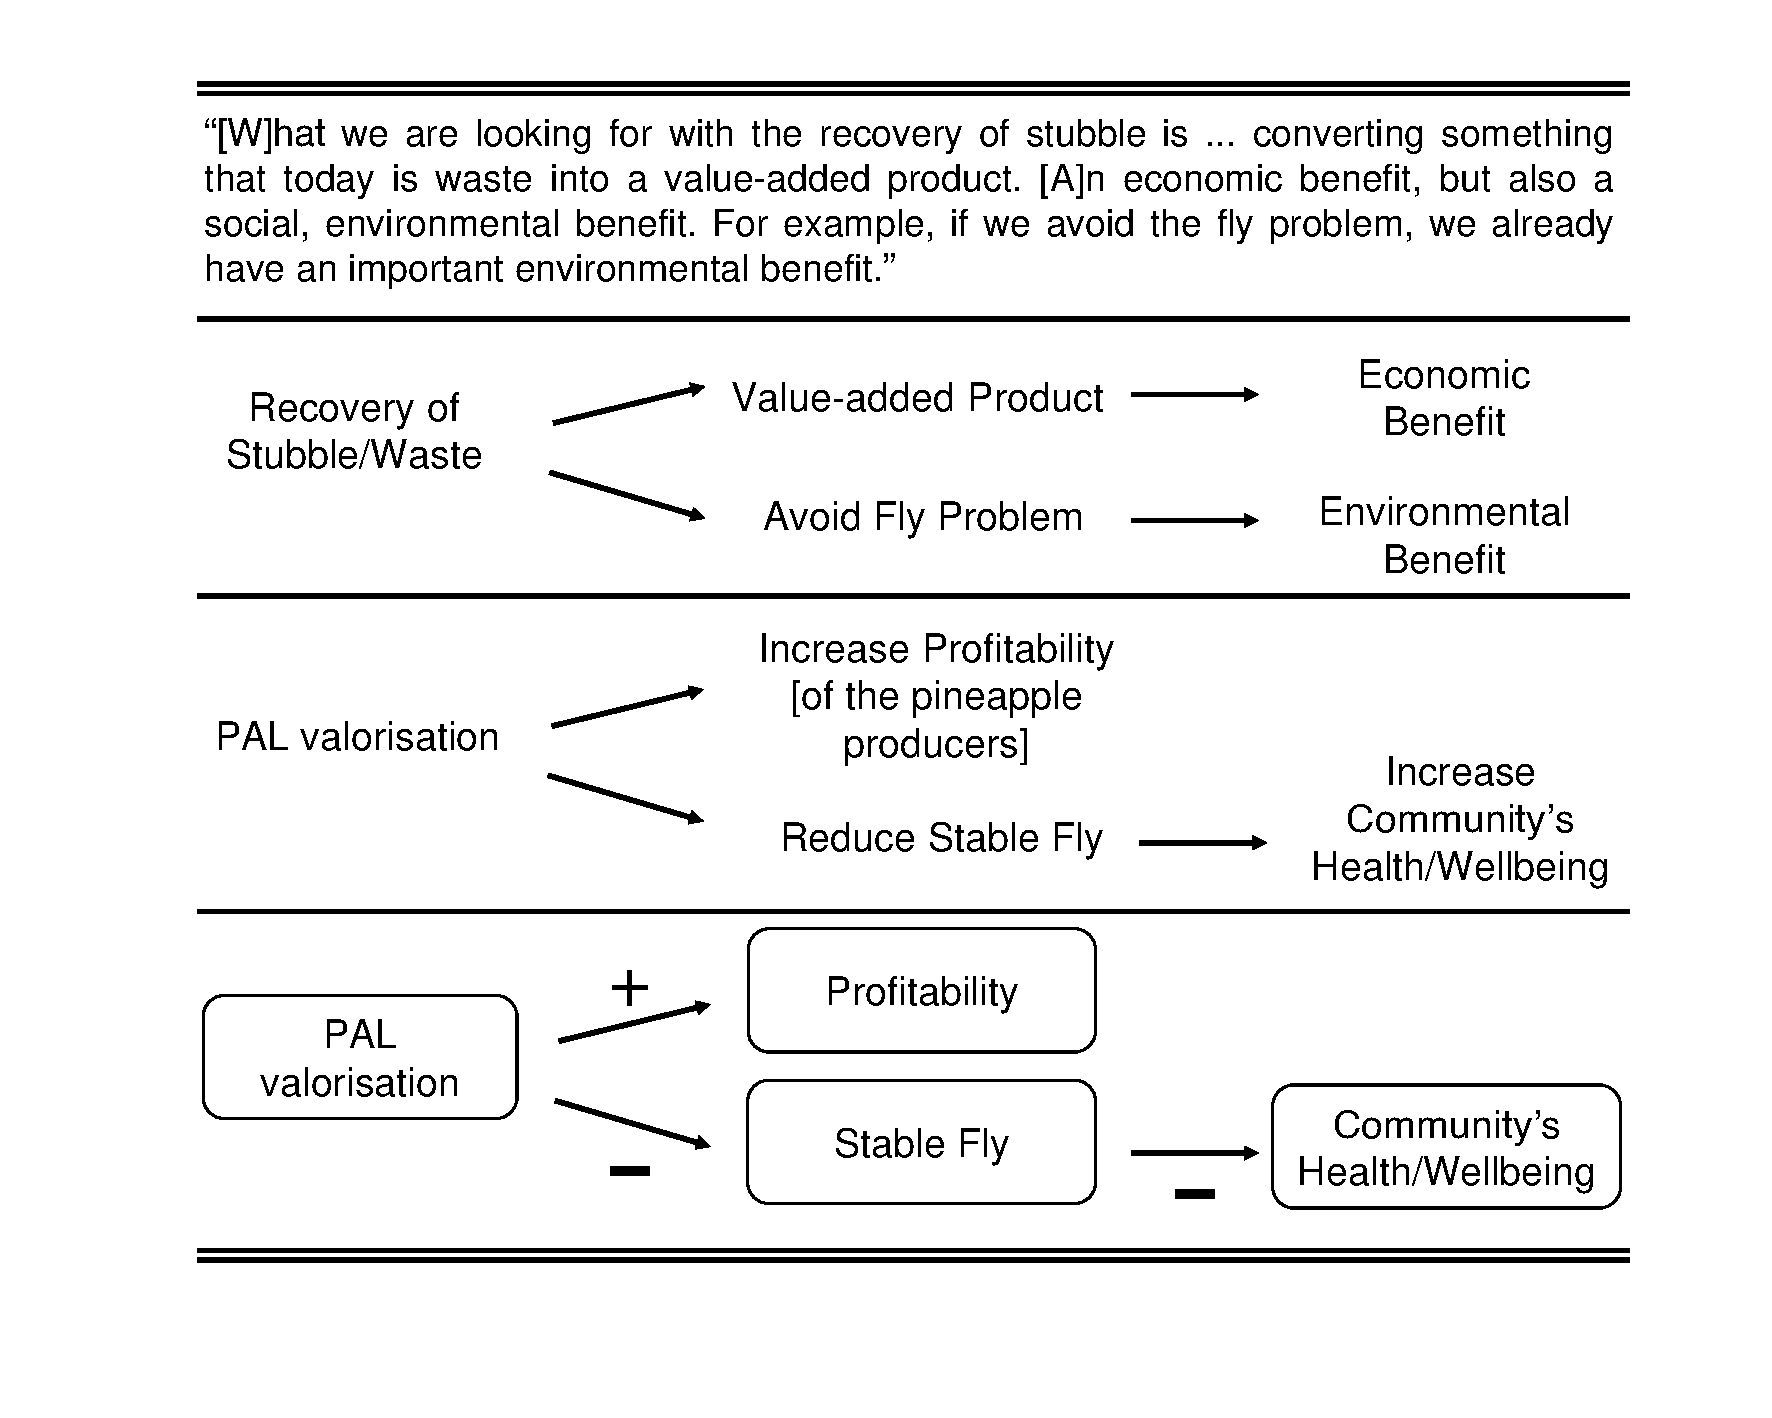
\includegraphics[width=\textwidth]{fig/processFCM.pdf}
\end{figure}


\subsection{Weighting connections}

After the concepts and connections are identified, the next step is to assign weights to the connections. For this purpose, a second round of participation from stakeholders is conducted using an online questionnaire. Qualtrics Online Survey Software was used to make the questionnaire form. For each connection, stakeholders were asked to assign a value to the strength they think exists between concepts. In the previous step, the sign of the connections was assigned based on what the majority of the statements from the interviews indicated. Thus, stakeholders were asked to indicate only the value of the connections. At the end of the questionnaire, respondents could comment on relationships or signs that they thought were incorrectly identified, or add new concepts and connections that they thought were missing. At this point, it is relevant to remind the reader that the FCM developed in this study is the so-called dynamical FCM, which means that the values represent the propagation of effects of one concept on another and not the measure of certainty that the stakeholder has of the connection. 

All the questions in the questionnaire followed the same structure ``If concept A increases, how much does concept B increase (decrease), on a scale from 1 to 5? (1 being increases (decreases) little and 5 being increases (decreases) a lot)". Initially, qualitative values --- Very High, High, Medium, Low, Very Low --- were used in the questionnaire, but it was soon realised that this, together with the sign of the connection, was confusing to respondents, and that a numerical scale, coupled with the terms increase and decrease to represent the sign of the connections, was simpler to interpret. The best way to formulate the questions is the one that works for the case and the target group, and examples of both qualitative and quantitative values can be found in the literature (e.g., see \cite{morone2021using} for the former and \cite{olazabal2016use} for the latter). A glossary containing all concepts and their definitions (see \cref{conceptsGlossary}) was provided with the questionnaire in case the respondents had doubts about what a concept term meant. At the end of the questionnaire, the output of the previous step, the visual map with all identified concepts and connections, was also provided to assist respondents in identifying missing concepts and connections. After four weeks of sending the questionnaire, the responses were collected to proceed with the final step in the process. 

\subsection{Quantitative aggregation}

For a comprehensive explanation of the quantitative aggregation process, we refer the reader to \cref{quantitativeAgg}

The data extracted from the questionnaire responses were transformed by converting the categorical ratings to an adjacency matrix. Sometimes, researchers use a scale to weigh the consistency of stakeholders' answers, giving more weight to experts who are believed to be more knowledgeable. In our case, we have assumed that all individual FCMs are equally valid and, thus, the same weight was applied to all maps when aggregating. 

With the aggregated matrix, we can perform a dynamic analysis of the FCM. As \cite{edwards2021building} mention, in a mathematical sense, the output of the analysis is static rather than dynamic, so they adopt the term ‘quasi-dynamic’ to indicate the dynamic character of the interpretation of the changes in the system. This quasi-dynamic analysis allows us to see where the system will go if things continue as they are, i.e., to determine the steady state of the system \citep{ozesmi2004ecological}. The steady-state value taken by each concept reflects its importance within the system according to stakeholders' knowledge and provides an idea of the evolution of the system in current circumstances \citep{lopolito2020combined}. 

To compute the steady state of the system, a vector of initial states of variables is first multiplied by the aggregated adjacency matrix of the FCM. Then, the resulting transformed vector is repeatedly multiplied by the adjacency matrix and transformed until the system converges to a steady state.  It is important to note that iterations are not related to time. This property allows an interpretation of the dynamics of the different factors relative to the other factors or relative to other descriptions of the system \citep{edwards2021building, diniz2015mapping}. In this sense, it is possible to evaluate different scenarios and outcomes by asking ``what-if" questions and simulating different conditions or policy choices. This can be used to compare what policy decisions or changes in the system would have the greatest effect on the variables of interest.

\section{Results and Discussion}

\subsection{Descriptive analysis}
\label{descriptiveFCM}

A total of 14 experts participated in the study. Three are classified as research related, one as government, and 10 as industry related. In the latter, we can find companies directly related to pineapple production and companies that are involved in PAL valorisation in some way. All stakeholders participated in the first round of participation, which consisted of one-to-one, in-person interviews. The online questionnaire, which took place in the second round of participation, was responded to by only half of the stakeholders. Four additional pineapple producers, two government agencies, and one company related to PAL valorisation were contacted to participate in the study, but no response was received. A list of stakeholders, their affiliation and role, and their participation in the participation rounds can be found in \cref{expertsList}.

\begin{table}[ht]
\centering
\resizebox{\textwidth}{!}{
\begin{threeparttable}
\caption{Profile, role and participation of stakeholders}
\label{expertsList}
\begin{tabular}{lcp{0.5\textwidth}cc} \hline \hline \\

Group & \begin{tabular}[c]{@{}c@{}}Respondent \\ Code\end{tabular}  & Role & \begin{tabular}[c]{@{}c@{}}Participation \\ in 1st round\end{tabular}  & \begin{tabular}[c]{@{}c@{}}Participation \\ in 2nd round\end{tabular}        \\ \hline
    Research & R1  & Works at university conducting research in  pineapple valorisation options      & Yes & Yes \\
                           & R2  &    Works at university conducting research in  pineapple valorisation options                                                                                              &               Yes        & Yes \\
                           & R3  & Agri-food research organisation involved in the design of an extraction machine                   &   Yes                    & No  \\ Government                 & G1  & Agency of the Ministry of Agriculture in charge of protecting agricultural resources from pests. &    Yes                   & No  \\
Industry & I1  & Small-scale farmer considering valorisation options                                              &           Yes            & Yes \\
                           & I2  & Large-scale farmer                                                                               &    Yes                   & No  \\
                           & I3  & Medium-scale farmer with various PAL valorisation projects                                       &    Yes                   & No  \\
                           & I4  & Large-scale farmer with a PAL valorisation business                                              &   Yes                    & Yes \\
                           & I5  & Large-scale farmer with a R\&D team researching valorisation options                             &    Yes                   & Yes \\
                           & I6  & Association of pineapple producers                                                               &      Yes                 & No  \\
                           & I7  & Company working on field extraction machine                                                      &     Yes                  & Yes \\
                           & I8  & Company marketing PAL as fodder                                                                  &      Yes                 & No  \\
                           & I9  & Company producing and marketing PALF                                                             &     Yes                  & No  \\
                           & I10 & State-owned enterprise that developed a PAL-based biogas plant                                                               &  Yes                     & No  \\ \cline{1-5} 
Number of participants  & & &  14 & 7 \\ \hline \hline
\end{tabular}
\end{threeparttable}%
}
\end{table}


The generation of knowledge by stakeholders in the interviews resulted in 32 concepts and 52 connections. The diagram representing the connections is presented in \cref{FCMdiagram}. A list with a description of the concepts, which was also shared with the stakeholders in the questionnaire, is shown in \cref{conceptsList}. A section to add comments was provided on the online questionnaire, and valuable feedback was given by three stakeholders. The stakeholders mentioned that some concepts were too broad and that narrowing the definition can make the connections clearer. They also mentioned a disagreement with the effect of the concept \textit{Profitability} on the concept \textit{Sustainability of the industry}; indeed, in the interviews, some stakeholders defined this relationship as positive, but the majority stated that it was negative. Finally, stakeholders emphasised the importance of transparency in the industry for the collection of data needed to conduct large-scale valorisation studies, and that the results of the small-scale studies that have been developed cannot be extrapolated. No further concepts or connections were added in this comment section. 

\newpage

\begin{landscape}
\begin{figure}[H]
\caption{FCM resulting from interviews}  
\label{FCMdiagram}
\centering
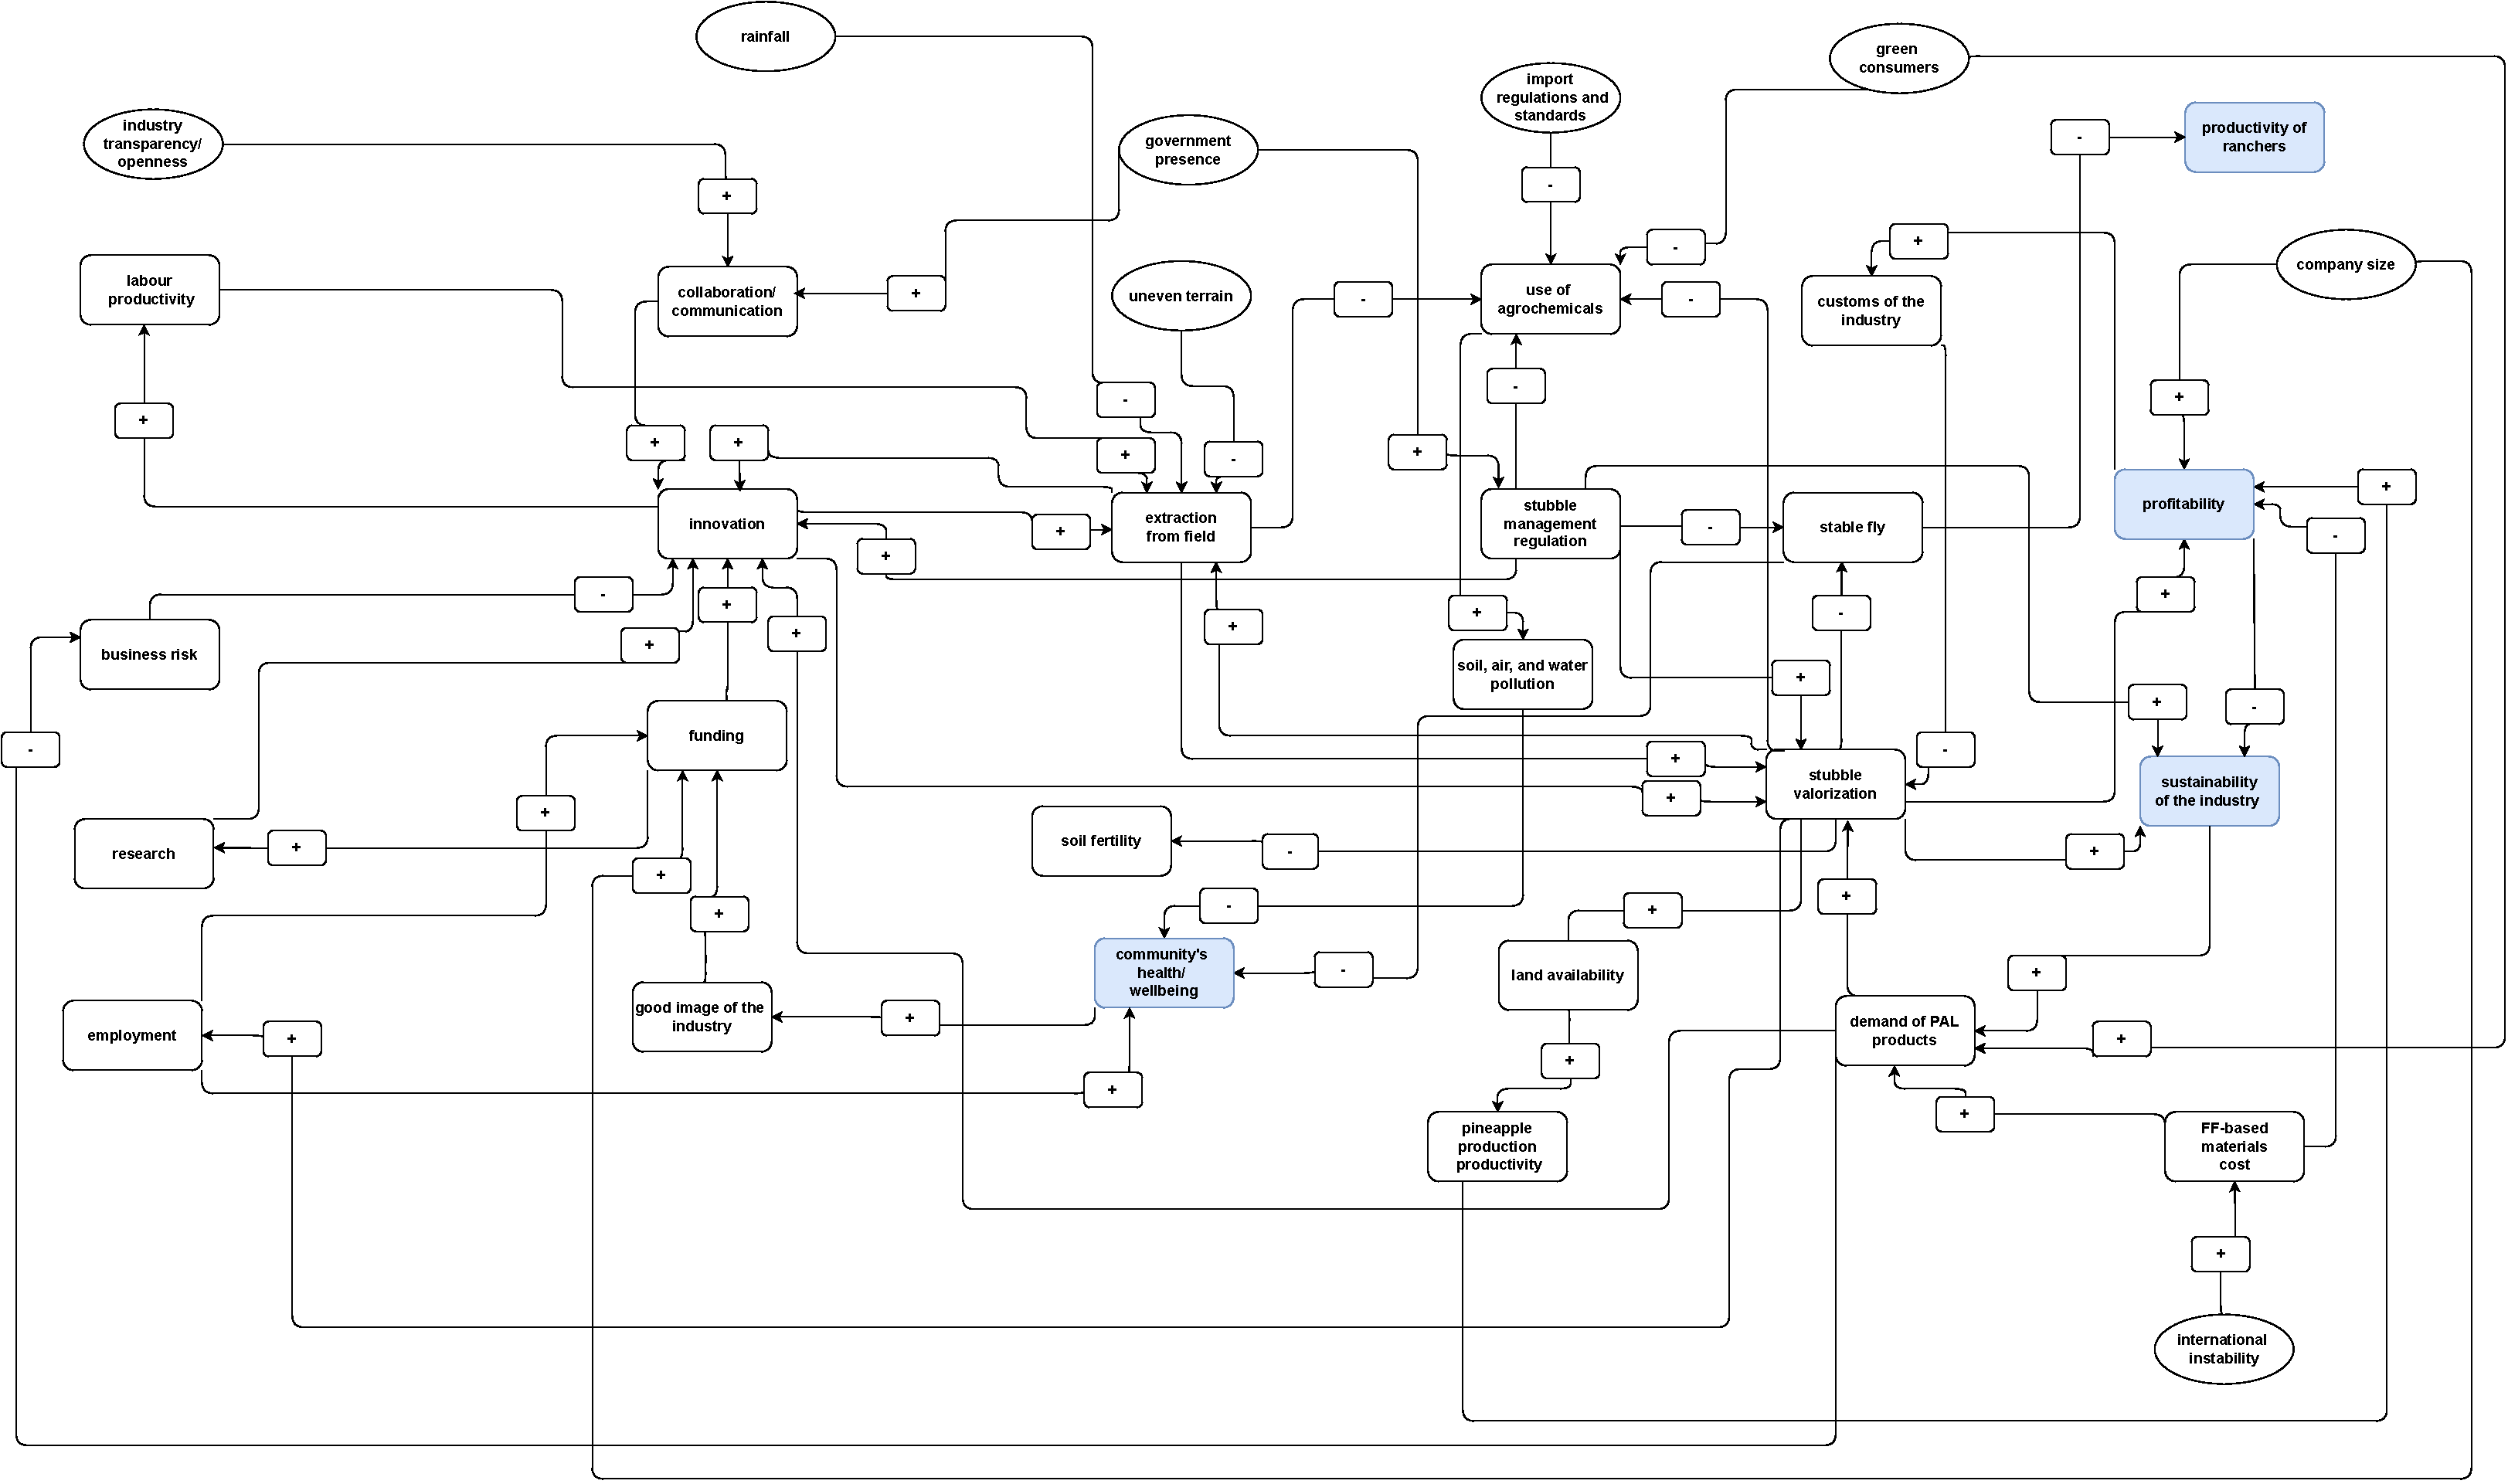
\includegraphics[width=23 cm]{fig/diagram.drawio.pdf}
\end{figure}
\end{landscape}

\clearpage

Most of the concepts were mentioned by more than one stakeholder. The most mentioned concepts, in addition to \textit{valorisation of PAL}, were \textit{Extraction from the field}, \textit{Innovation}, \textit{Use of agrochemicals}, and \textit{Government presence}. The least mentioned concepts are \textit{Ranchers' productivity}, \textit{Soil fertility}, and \textit{International instability}. It is also useful to look at the entropy, defined as 

\begin{equation}
\label{entropyEq}
E(R) = - \sum_{i=1}^{11} p_i \times log_2(p_i),   
\end{equation}

for a relationship \textit{R}, where $p_i$ is the proportion of responses (per linguistic term) to the causal relationship between two concepts. As an example, take the entropy for the effect of \textit{PAL valorisation} on \textit{Sustainability of the industry}. For this relationship, one linguistic term was chosen by three respondents, another two terms were chosen by two respondents each, and the remaining eight terms were not chosen. This translates to $1 \times (- \frac{3}{7} \times log_2(\frac{3}{7})) + 2 \times (- \frac{2}{7} \times log_2(\frac{2}{7})) = 1.50 $ . The larger the entropy, the less agreement there is between experts on a particular relationship. Of the 52 connections in the FCM,  \textit{Collaboration/Communication} on \textit{Innovation} was the connection with the lowest entropy (0.954), and \textit{Labour Productivity} to \textit{Extraction from the field} and \textit{Stubble Management Regulation} to \textit{Agrochemicals Use} the two with the highest entropy (2.50). The median and the mean of the entropy values are 1.75 and 1.79 respectively. 

It is also valuable to describe the structure of the FCM using graph theory and network analysis. Specifically, we can look at the network density, the in-degree and out-degree, and the centrality of the network. The density tells us how closely the concepts are connected in the network. In-degree and out-degree measurements represent the total weight of relations that enter and exit a particular concept. Finally, centrality represents the sum of in- and out-degrees, determining the role of the individual variables within the system.

The network density can be calculated easily, it is simply the number of connections in the system over the potential connections. The network density of our FCM is $52/\frac{32\times31}{2}=0.104$, i.e.,  a density of 10.4\%. \cite{ozesmi2004ecological} note that a low density indicates that interviewees see a low number of causal relationships among concepts, which translates into fewer options to change things in the system, and \cite{jetter2014fuzzy} explain that it can be interpreted as an undesirable loss of information on connections or as a desirable focus on less but truly important connections. The out-degree and in-degree indices are presented in \cref{degreeFCM}. In descending order, the most influenced variables in the system are \textit{Innovation}, \textit{Extraction from Field}, and \textit{PAL valorisation}. Similarly, the most influential variables are \textit{PAL valorisation}, \textit{Stubble Management Regulation}, and \textit{Innovation}. Since \textit{Innovation} and \textit{PAL valorisation} have large in-degree and out-degree indices, they are considered important in the transition process of the system.  

There are eight ``senders", i.e., variables with zero in-degree and positive out-degree, meaning that their role is to stimulate the rest of the system. The senders are represented by a circle in \cref{FCMdiagram}. It is relevant to note that senders are generally used as policy drivers for intervention scenarios \citep{morone2021using}.  In our case, we consider the following concepts as policy drivers: \textit{Green Consumers}, \textit{Government Presence}, \textit{Import Regulations}, and \textit{Industry Transparency}. From these policy variables, government presence and Green Consumers have the largest out-degree value, meaning that they can have the largest impact on the system. Similarly, there are two \textit{receivers}, variables with positive in-degree and zero out-degree, they receive input from other variables and can be used as final monitors of the system. The two receivers are \textit{Soil Fertility} and \textit{Ranchers productivity}. The rest of the variables, those with non-zero in-degree and out-degree, are “transmitters”, and keep the system connected. Usually, receivers are outcome variables; they reflect the response of the system to interventions. In our case, the outcome variables can be both receivers and transmitters, and they are \textit{Ranchers productivity, Pineapple Producers' Profitability, Community's Health/Wellbeing}, and \textit{Industry Sustainability}. These outcome variables are represented with blue boxes in the \cref{FCMdiagram}.


\begin{table}[H]
\centering
\resizebox{\textwidth}{!}{
\begin{threeparttable}
\caption[Network analysis indices \& results]{Network analysis indices \& results of the baseline quasi-dynamic analysis}
\label{degreeFCM}
\begin{tabular}{lcccc} \hline \hline
Variable & In-degree & Out-degree & Centrality & Steady state value\\ \hline
innovation                 &      4.44 &       2.02 &        6.45 &    0.97 \\
fieldExtraction            &      3.22 &       1.96 &        5.18 &    0.94 \\
palvalorisation            &      3.19 &       4.69 &        7.88 &    0.94 \\
funding                    &      1.79 &       1.27 &        3.07 &    0.85 \\
palProductsDemand          &      1.77 &       1.83 &        3.60 &    0.85 \\
pineappleProdProfitability &      2.39 &       0.98 &        3.37 &    0.82 \\
laborProductivity          &      0.66 &       0.57 &        1.23 &    0.81 \\
industrySustainability     &      1.75 &       0.60 &        2.35 &    0.81 \\
landAvailable              &      0.64 &       0.53 &        1.17 &    0.80 \\
academia                   &      0.67 &       0.60 &        1.27 &    0.80 \\
employment                 &      0.50 &       1.25 &        1.75 &    0.78 \\
industryImage              &      0.79 &       0.53 &        1.32 &    0.77 \\
businessRisk               &      0.50 &       0.54 &        1.04 &    0.77 \\
pineappleProdProductivity  &      0.53 &       0.62 &        1.14 &    0.77 \\
industryCustoms            &      0.50 &       0.60 &        1.10 &    0.76 \\
pollution                  &      0.75 &       0.74 &        1.49 &    0.70 \\
collabComms                &      1.28 &       0.77 &        2.04 &    0.66 \\
stubbleMgmtRegulation      &      0.69 &       2.98 &        3.68 &    0.66 \\
costFFmaterials            &      0.57 &       1.08 &        1.65 &    0.66 \\
ranchersProductivity       &      0.71 &       0.00 &        0.71 &    0.58 \\
communityHealth            &      2.15 &       0.79 &        2.93 &    0.57 \\
soilFertil                 &      0.37 &       0.00 &        0.37 &    0.55 \\
stableFly                  &      1.16 &       1.48 &        2.63 &    0.36 \\
agrochemicalsUse           &      3.03 &       0.75 &        3.78 &    0.20 \\
companySize                &      0.00 &       1.30 &        1.30 &    0.00 \\
govtPresence               &      0.00 &       1.36 &        1.36 &    0.00 \\
importRegulations          &      0.00 &       0.68 &        0.68 &    0.00 \\
industryTransparency       &      0.00 &       0.61 &        0.61 &    0.00 \\
rain                       &      0.00 &       0.61 &        0.61 &    0.00 \\
unevenTerrain              &      0.00 &       0.60 &        0.60 &    0.00 \\
intInstability             &      0.00 &       0.57 &        0.57 &    0.00 \\
greenConsumers             &      0.00 &       1.13 &        1.13 &    0.00 \\
 \hline \hline
\end{tabular}
\end{threeparttable}%
}
\end{table}

\subsection{FCM model and fuzzy inference}

The interpretation of FCM outputs from the quasi-dynamic analysis is done by comparing the steady-state values of concepts after stabilisation. The steady state was achieved in the 10th iteration, as shown in \cref{outputFCM0}. This output reflects the current perception of stakeholders about the pineapple sector in Costa Rica in the context of circularity driven by PAL valorisation. As expected, the drivers of the model go to zero. We added a self-reinforcing relationship to the matrix, as recommended by \cite{diniz2015mapping}, but the steady state of the remaining variables did not change and the drivers reached the same value, not providing additional information. Most variables' steady-state corresponds to their centrality, i.e., those with high centrality also have a large steady-state value. However, some observations are in order. \textit{Collaboration/Communication, Stubble Management Regulation, Community's Health, Stable Fly} and \textit{Agrochemicals Use} are all relatively low compared to other variables with similar centrality, and \textit{Labour Productivity}, on the contrary, presents a relatively high steady-state value. It is also important to note that the transmitters with the highest values, apart from the obvious and central ones (\textit{innovation}, \textit{field extraction}, and \textit{PAL valorisation}), are \textit{Funding}, \textit{Labour Productivity}, and \textit{Academia}. 


\begin{figure}[H]
\caption[Output of the quasi-dynamic analysis]{The output of the quasi-dynamic analysis. The output for 11 concepts that go to zero is not shown.}  
\label{outputFCM0}
\centering
\includesvg[width=\textwidth]{fig/naturalSimulation.svg}
\end{figure}


\subsection{Drivers' intervention simulation}

The baseline output is useful to analyse what stakeholders believe is the unaltered result of the system's dynamic. This does not mean, for example, that the large values of \textit{Innovation} necessarily translate to a current situation of extensive innovation. Instead, it tells us that \textit{Innovation} is the central variable in the context of circularity and sustainability in the pineapple sector in CR. As such, we find it interesting and useful to analyse scenarios in which drivers are modified from the initial weights defined by stakeholders to see how the outcome variables react. We run the dynamic analysis under four different scenarios and compare the results in \cref{interTable}. Usually, scenarios are built by either modifying the initial values of the concepts (single-shot interventions) or by introducing a new concept in the initial FCM and defining the connection weight that it has on the target concepts (continuous interventions). We tested both types of scenario implementations and found no significant differences. The values shown are for the continuous interventions' implementation. In addition to the individual interventions, we run simulations with mixed interventions to see if there is a different effect when joining the stimuli of two drivers. The effect on the outcome variables for the individual interventions and the mixed interventions is depicted in \cref{interBars}.


\begin{figure}[ht]
\caption[Impact of interventions on outcome variables]{Impact of interventions on outcome variables (\% Change from steady state of baseline)} 
\label{interTable}
\centering
\includesvg[width=\textwidth]{fig/interventionTable.svg}
\end{figure}


The intervention in \textit{Government presence} had the most significant effect on all four outcome variables by far, \textit{Industry Sustainability} receiving the largest impact, followed by \textit{Community's Health/Wellbeing}. The drivers \textit{Import regulations} and \textit{Green Consumers} also had a significant impact on \textit{Community's Health/Wellbeing}. The outcome variable that was less affected by single interventions was \textit{Profitability of the pineapple producers}. The intervention of \textit{Import regulations} only had a small effect on \textit{Community's Health/Wellbeing}, and the intervention of \textit{Industry's Transparency} had a negligible effect on the outcome variables.  

Analysing \cref{interTable}, we notice that the effect of single interventions on transmitters was more heterogeneous than on receivers. The driver that affected more transmitters was \textit{Government presence}, followed by \textit{Green Consumers}. The transmitters affected the most were \textit{Agrochemical use}, \textit{Pollution}, and \textit{Collaboration/Communication}. The latter is only affected by \textit{Government presence} and \textit{Industry Transparency}, not by the intervention of \textit{Import Regulations} and \textit{Green consumers}. Interestingly, these two drivers reduce \textit{Pollution} significantly, which tells us that even though stakeholders believe that greater government participation and industry transparency can improve collaboration, it would not significantly reduce pollution. Only regulations imposed by importing countries and consumer preferences can change the behaviour of producers and, consequently, the level of pollution. These claims are supported by the literature, although with some caveats. \cite{sajjad2015sustainable} explain that inadequate government support is one of the barriers to the implementation of sustainable supply chain management. As stated in a report by the \cite{oecd2017oecd}, this is the case in the Costa Rican agricultural sector, in which a fragmented 
institutional structure obstructs the coordination of actions and policy objectives. Furthermore, the report acknowledges the deficit in the technical capacity of the agricultural public sector and its investment restrictions due to the intensification of budget restrictions since 2013. As regards consumer preferences, the benefits of going green -- increased efficiency in resource use, increased sales, development of new markets, improved corporate image and enhanced competitive advantage--- are understood by companies \citep{dangelico2010mainstreaming}. Regarding import regulations, the evidence is mixed, but \cite{montiel2019effect} notes that the expansion of certifications creates uncertainties for producers that consequently reduce their readiness to adopt any standard.

\begin{figure}[ht]
\caption{Impact of (mixed) interventions on outcome variables} \label{interBars}
\begin{subfigure}[b]{0.45\textwidth}
  \centering
  \includesvg[width=\textwidth]{fig/interventionBar.svg}
\caption{Impact of interventions on outcome variables} 
  \label{interventionBar}
\end{subfigure}%
  \hfill
\begin{subfigure}[b]{0.45\textwidth}
  \centering
  \includesvg[width=\textwidth]{fig/mixesOutput.svg}
\caption{Impact of Mixed Interventions on Outcome Variables}    
  \label{mixedBar}
\end{subfigure}
%\captionsetup{justification   = raggedright, singlelinecheck = false}
\end{figure}

We can also observe that the effect of \textit{Import regulations} and \textit{Green Consumers} on \textit{Community's Health/Wellbeing} is channelled through the reduction of \textit{Agrochemical Use}, while that of \textit{Government Presence} is channelled through two transmitters, \textit{Stubble management regulation} and \textit{Agrochemical Use}. We also find it interesting to note the negative impact on \textit{Business Risk} due to the intervention on \textit{Green consumers}. The direct connection between the concepts, which makes this impact large, is due to stakeholders indicating that \textit{Business Risk} is one of the main factors preventing investment in innovation related to PAL extraction and innovation. This is reasonable, as one of the main barriers in the development of sustainability strategies is the uncertainty about market demand \citep{chkanikova2015corporate}. Therefore, we can see how more green consumption, which increases the demand for PAL products, alleviates this uncertainty and reduces business risk. 

Regarding mixed interventions, the first thing that strikes us when we look at \cref{mixedBar} is the greater effect that a combination of drivers can have on outcome variables. The effect of the first three mixes can be attributed mainly to \textit{Government Presence}. The effect of the other three intervention mixes is almost negligible, except for the case of \textit{Community's Health/Wellbeing}. The combination of \textit{Government Presence} and \textit{Green Consumers} brings the greatest benefit to all outcome variables, highlighting how the influence of market demand and regulations can ensure collaboration and reduce unsustainable practices at the same time. On the other hand, a relevant remark is that the percentage change from the steady-state values attributed to these mixes is not much greater than the changes attributed to the single interventions. For example, the mixture of \textit{Import Regulation} and \textit{Green Consumers} results in a change of 1.11\% from the steady state value of \textit{Community's Health}, whereas the changes from intervening these variables alone are 0.86\% and 0.75\%, respectively. This is relevant, for instance, when deciding what policies or changes should be prioritised to attain sustainability in the industry and for companies to know how external factors can affect their business. 


\subsection{Bringing it all together}

Stakeholders modelled PAL valorisation as a transmitter, which means that it is the means to an end, it has to be ``activated" by a driver of change in the system. Thus, it is challenging to understand how it can be enhanced to increase the impact on outcome variables. PAL valorisation can have a positive effect by substituting the use of agrochemicals, increasing employment, generating additional profit for producers, and improving the image of the industry. Its impacts can be relevant and long-lasting, but they are channelled less directly than regulations. 

For example, the prohibition of an agrochemical for pineapple exporters has a simple and tangible effect, and its drivers and outcomes are trivial. On the other hand, the drivers of change needed to valorise PAL, a valid alternative to agrochemical use, are less clear and its consequences are more dispersed throughout the system. From the model of production viewpoint, as discussed in \cref{theoryframe}, the use of agrochemicals in the linear economy only serves to maximise profits and minimise other resources, such as water or labour. But PAL valorisation in the context of CB must meet more criteria, such as reducing waste (almost) completely and creating value-added products. Moreover, if we consider the characteristics of CB in the agricultural sector, the PAL valorisation practices should also account for the regeneration and biodiversity of the ecosystem that surrounds it. 

\paragraph{Barriers}\mbox{}\\
At this point, we find it useful to try to answer the research questions defined in \cref{researchQ}. The initial question we proposed was
\textit{What are the cultural, financial, market-related, operational, and technological barriers preventing the valorisation of pineapple stubble in Costa Rica?}. These barrier categories were tailored to the industry and country conditions, but they have similarities to those defined by \cite{gottinger2020studying} and summarised in \cref{theoryframe}. As these categories are commonly used when analysing the transition towards a circular bioeconomy, delineating our discussion around them can help make comparisons in future research. The categories used below are Policy and Regulation, Technology and Materials, Market and Investment, Knowledge and Networks, and Sectoral Routines and Structures. 

First, we attempt to comment on the cultural aspects, which fall into the category of \textit{Sectoral Routines and Structures}. Stakeholders view the customs of the industry as an impediment to valorising PAL. The customs of the industry are the inherited practices that prevail in the industry, such as the use of agrochemicals, monoculture, and productivity maximisation. These practices degrade the environment and do not align with sustainable practices \citep{magdoff2000hungry}. Moreover, most stakeholders imply that larger companies present larger profits and that as profits increase, unsustainable customs are reinforced. A systematic assessment of 118 studies explains that there is no conclusive evidence for a relationship between farm size and resource use efficiency, GHG emissions, or profit \citep{ricciardi2021higher}. However, small and medium-sized pineapple producers in Costa Rica have progressively been replaced by corporate farmers, who also benefit from larger profits \citep{rodriguez2020extractivismo}. Ultimately, the nature of the structure of the pineapple industry in Costa Rica--big corporations, monocropping, and productivity maximisation---incentivises less sustainable customs, which hinder the development of PAL valorisation as an alternative to current practices. 

The technologies required to extract PAL from the field and transform it into value-added products are not fully developed. Stakeholders indicated that large corporations are generally more able to access international and domestic investment, but small- and medium-scale farmers usually do not own machinery and cannot afford to invest in innovation. Moreover, financial barriers are not related to access to funding per se, i.e., availability of funds. Instead, the barriers to funding relate to the mobilisation of investment resources. Although these considerations fall partially on the \textit{Market and Investment Conditions} category of barriers, the need to coordinate how much of the available funding is allocated to innovation and who should provide such funds shifts the financial barrier into a collaboration barrier. 

Each stakeholder---experts from the industry, the academia, and the government---has a different view about what roles each other should play in the PAL valorisation process and who should initiate the required change. Testing at scale the different PAL valorisation options is still rare. Collaboration in technical and business model innovation is still required to share the potential risks and costs and to get out of the experimental phase. Moreover, risk-averse attitudes are a common obstacle to transitioning towards CB. Stakeholders usually disagree on who should provide the initial funds and take on the business risk. Moreover, there is no consensus on what the role of the government should be to channel funds. The lack of collaboration and the risk-averse attitude reinforce each other and create a combination of \textit{Knowledge and Network} and \textit{Sectoral Routines and Structures} barriers.

The technological barriers that prevent PAL valorisation are closely related to operational barriers. In the \textit{Technology and Materials} barriers category, we identify the uneven terrain that is commonly present in pineapple fields as an operational barrier to extracting PAL from the field efficiently. Rainfall is another factor that, coupled with the uneven terrain, makes it very difficult to manoeuvre large machinery in the field. To this day no machine can extract PAL without additional human labour in Costa Rica. As regards the valorisation options, there are several technologies to make value-added products (see \cref{valoriseOptions}). However, stakeholders commonly mention that it is difficult to obtain input material to conduct large-scale projects. Due to these operational barriers and the aversion to business risk mentioned above, valorisation research projects do not take place at a sufficiently large scale to extrapolate the results. This barrier is easily understood by producers and people working closely with the logistical aspects of the business, but it can be less frequently identified by researchers and policymakers. 

\paragraph{Drivers of Change} \mbox{}\\
As we describe the barriers preventing the valorisation of PAL, it is natural to ask \textit{What is needed to overcome these barriers? Whose action is required?} First, stakeholders agree on the strong effect that collaboration and communication have on innovation. Moreover, our results indicate that government agencies are seen as a potential intermediary capable of coordinating collaboration between the industry, international organisations and research institutions. Although some experts identified policy and regulation barriers, such as a lack of technology-push policies, most of them perceive public agencies as potential drivers of change. However, from the government's side, agencies of the Ministry of Agriculture are mostly concerned with problems caused by the stable fly and stubble management practices. Thus, their coordination efforts are not directly focused on PAL valorisation, which is seen as just another stubble management alternative. Finally, although stakeholders identify the government as the necessary mediator, they acknowledge its lack of resources to monitor and lead a transformation in the industry structure. 

Another driver influencing collaboration and communication in the FCM is the transparency and openness of the industry. The simple idea that transparency about supply chains and openness of companies can help reduce environmental impacts is widely accepted \citep{kashmanian2017building, jahansoozi2006organization}. Simply put, transparency and openness prevent duplicated efforts to find PAL valorisation solutions. Unfortunately, we identify a contradiction as companies want to share but also protect knowledge. If companies are open not only about their practices but also about their findings and innovations, collaboration is magnified to accelerate progress towards a common solution.

As observed in the interviews, the subject of PAL valorisation has been conducted predominantly in academia, with few companies investing in experiments. As documented in \cref{neweconomy}, researchers have extensively studied the properties of PAL to assess the valorisation options. However, little research has focused on the operational and socioeconomic aspects of the process needed to valorise PAL at a large scale. Producers mentioned the importance of academia in bringing about innovation and stressed the importance of collaborating to carry out PAL valorisation projects. For researchers, on the other hand, funding is a shared concern. In this sense, it is of the utmost importance to facilitate collaboration between researchers and companies with sufficient resources to undertake projects at a large scale. This would eliminate barriers in two groups, namely \textit{Market and Investment Conditions} and \textit{Technology and Material}. Additionally, knowledge from engineering companies and industries with similar supply chains to those of the pineapple can help find PAL extraction solutions. Finally, partnerships with development aid agencies and environmental organisations interested in participating in sustainability programmes can take over those tasks that government agencies cannot.

\paragraph{Benefits of PAL valorisation} \mbox{}\\
After analysing the barriers to PAL valorisation and the actions needed to overcome them, one last question emerges: \textit{What are the benefits and challenges of valorising the stubble?}. Although most benefits of PAL valorisation were mentioned by all stakeholders, there is a large disagreement on the effect of PAL valorisation on the use of agrochemicals, the stable fly, and the profitability of producers. Let us analyse these three connections. First, because agrochemicals are not only used for stubble management but also to control pests, produce artificial ripening, and enhance fruit size, stakeholders view the potential of PAL valorisation to reduce agrochemicals as limited. 

More surprising is the disagreement regarding the presence of the stable fly. The fly reproduces in the decomposing pineapple stubble after harvest; if the PAL is extracted and the remaining low-volume stubble is incorporated into the soil, the probability of stable fly reproduction is reduced significantly. A better understanding of the reasons for this disagreement is needed. Finally, the connection between PAL valorisation and profitability occurs for three reasons, (1) profits from value-added products; (2) cost reductions from current stubble management practices; and (3) earlier next plantation. Although some stakeholders do not identify these benefits, most agree with the general idea that PAL valorisation can increase sustainability. Thus, information campaigns can increase the awareness of producers about the specific economic benefits of PAL valorisation.

\paragraph{Challenges}\mbox{}\\
When we think of the challenges to valorise PAL systematically, we immediately think of the title of this chapter. Harvesting The Fruits of Uncertainty refers to the complexity and fuzziness of the problem under study, but also to its challenges and possibilities. Challenges refer to milestones that need to be achieved, and, in a way, they provide a more positive perspective than barriers. Overcoming or adapting to uncertainty is one of the biggest challenges we identify in the study, which is translated into the business risk concept. The unpredictability of the market demand for bio-based products is one of the main challenges to investing in solutions. An increase in green consumerism can reduce uncertainty, as shown in \cref{mixedBar}, but more market research is needed to incentivise investment in PAL-valorisation solutions. 

Another challenge is the introduction and changes in standards and regulations related to bio-based products, biofuels, and bioenergy. Efforts to identify market demand and applicable regulations can provide clearer prospects for the potential of PAL-based products. Another clear challenge is to attain a collaborative network of producers, researchers, government agencies, and investors that exchange knowledge and share risks and successes. Finally, it is worth mentioning a technical challenge, the consequences of stubble extraction on soil fertility, which have not been quantified as of now. Stubble generates several environmental problems when managed in the field, but it also provides nutrients to the soil when incorporated into it. As PAL starts to be extracted, soil fertility can be reduced, affecting farmer productivity. If it turns out that the effects of systematic extraction are significant, pineapple producers will have to find solutions that do not require the additional use of agrochemicals. 

\section{Conclusion, Limitations, and Recommendations}

In this chapter, we have discussed the theories on the transition towards a circular (bio)economy (CB) and Circular-Oriented Innovation (COI) relevant to the subject of Pineapple Leaves (PAL) valorisation. Using the Fuzzy Cognitive Mapping (FCM) method, we structured and elicited the knowledge gathered through interviews with stakeholders working in or collaborating with the pineapple industry in Costa Rica. Our results indicate that despite the increasing research in the last two decades, PAL valorisation businesses are still rare and awareness of its possibilities and benefits is low among producers. 

We found the main barriers preventing the adoption of PAL valorisation practices, which we analysed using a common categorisation criterion in studies of circular bioeconomy. The main barriers discussed include the unsustainable practices embedded in the industry, the (mis)allocation of funds for innovation, risk-averse attitudes, lack of collaboration, the topographic features present in the pineapple fields, and the lack of large-scale research projects. 

Regarding the drivers of change, most stakeholders view government agencies as potential mediators, instead of generators of barriers. Moreover, transparency and openness can drive more and better collaboration, but producers and innovators show a contradiction in their desire to collaborate. Greater transparency would help transfer knowledge, avoid duplication of efforts, and share risks. Additionally, we find that researchers are seen as relevant actors in driving circular-oriented innovation, but more funding and collaboration are needed to conduct large-scale projects and research focused on the operational and socioeconomic aspects of the process. Finally, partnerships with development aid agencies can help raise the support and funding that the local government cannot provide. 

As for the benefits of valorising PAL, the reduction of the stable fly is contested by some interviewees. More research on this disagreement would be useful to understand its causes. Another benefit identified is the reduction in agrochemicals, which is limited due to their use in other pineapple production processes. Finally, the financial benefits of valorising PAL are not acknowledged by all stakeholders. Thus, raising awareness of the socioeconomic benefits of PAL valorisation is required to motivate potential investors.

Our results emphasise the early stage of development of PAL valorisation in Costa Rica. However, the theories on COI illustrate that the barriers faced by the industry are common in CB transitions. As recommended by \cite{blomsma2022making}, we conclude that it would be useful to take a sufficiently long time horizon to understand circular phenomena in the industry. Periodic analyses by researchers to compare the evolution of the transition can shed light on features that are not identified in a one-time study. Regarding stakeholders and policymakers, we recommend looking at challenges that can be achieved instead of barriers that may not be overcome. Market research and a better understanding of the regulations regarding PAL-based solutions would provide clearer opportunities. Additionally, every actor in the system can and should connect and create tighter and stronger collaborative networks. The transition towards a CB in the agricultural sector is not a one-day or one-person effort, but a collection of milestones achieved by collaboration throughout time. 

Finally, we find it relevant to mention several limitations and considerations of the study. The use of interviews helps in understanding the subject under study in-depth but limits the extent to which results from the analysis can be extrapolated. In some cases, the results are corroborated by the literature and theory, but sometimes they are distinctive of the area under study. Regarding the use of FCM to elicit knowledge, although stakeholders create connections, the researcher ultimately decides how the map is constructed. In this sense, it is important to pay attention to potential biases and errors that may arise in the modelling process. For example, missing connections that are true by construction but were not mentioned in the interviews were later identified, such as the effect of agrochemical use on the stable fly. In this sense, we recommend that researchers complement the interviews with a literature review to add essential connections to the system (see \citep{edwards2021building}). Aside from these considerations, we find the FCM method useful for organising and identifying fuzzy knowledge, especially in the case of unexplored or developing phenomena.

The collection of information in two stages, using one-to-one interviews and an online questionnaire, proved relatively inefficient, with a low response rate in the latter. We believe this is related to stakeholders in the agricultural sector being used to working outdoors and with dynamic routines. Moreover, aggregating contrary views and simplifying a qualitatively modelled complex system can be challenging for the researcher. In this sense, we recommend using in-person workshops to motivate participation and reach agreements about complex connections. Finally, the selection of interviewees is a clear bias in the information collection, as they were selected because of their relation to PAL valorisation activities. If we were to interview pineapple producers who are not aware of this process, we would perhaps gather less information, but also very useful and valid viewpoints. Finally, as more is understood about the structure of the PAL valorisation industry in Costa Rica, the use of a theoretical framework focused on circular bioeconomy transitions, such as the Technological Innovation Systems, can prove useful in carrying out periodic studies that can track progress throughout time in an organised manner. 
